\section{Evaluation}
\label{sec:eval}

We present an evaluation study of our runtime-assisted approach to
convergent RDTs with help of our prototype \quark implementation. The
benchmark we chose for the study is a collaborative document editing
application -- a common usecase addressed by several CRDT
proposals~\cite{rga, treedoc, crdts}. However, unlike these
other approaches, we did not have to build a dedicated replicated data
type to represent collaboratively-edited documents; an ordinary
document format extended with a merge operation would suffice. While
many data structures exist to represent text documents (e.g.,
ropes~\cite{boehm95}), we decided to adopt the simplest representation
of a document as a list of characters. 
\begin{center}
\begin{ocaml}
        type doc = char list
\end{ocaml}
\end{center}
While being simple, the advantage of this presentation is that we can
simply reuse the three-way \C{List.merge} function of the list data
type to merge documents. \C{List.merge} is a simple implementation of
the GNU \C{diff3} algorithm~\cite{gnudiff} in ~60 lines of OCaml. We
thus adopt a straightforward approach to building a collaborative
document editor with the intention to keep the development effort low
enough to be easily replicated. The convergence guarantee of \quark
ensures that the simplicity of our implementation doesn't come at the
expense of correctness. We now describe an evaluation that
demonstrates that it also doesn't come at the expense of the editor
performance.

Our experiment setup consists of multiple collaborators simultaneously
editing a 10000+ line document obtained from the Canterbury
Corpus~\cite{canterbury}. Each user holds a replica of the document
and is assumed to be editing the document at the speed of 240
characters per minute or 1 character every 0.25s. At 6 characters per
word, this amounts to 40 words per minute, which is the average typing
speed of humans. Each edit is immediately persisted to the disk by
creating a new version in the backing store. Thus there are at least
as many versions of the document as there are edits. Such extensive
versioning may be considered excessive in practice and could be
disabled. Each user process runs a \quark thread that commits
user-generated document versions to the local branch, while
merging with the concurrent versions from the remote branches in the
background. Each merge is synchronized as described in previous
sections.

\quark's background merges however pose a new problem as they create
new versions on the local branch in the background while the user is
busy editing an older version. When the user attempts to write their
version of the document to the store, simply committing it would
effectively override the concurrent updates from other users obtained
via background merges. The solution, fortunately, is straightforward:
we \emph{merge} the user-submitted value with the (value of) the
latest version on the local branch to create a new version that
includes the updates from either direction. 
% The LCA for this merge is
% simply the last version on the local branch read by the user. This
% merge need not be synchronized as it doesn't alter the LCAs between
% any two branches. The merged value can then returned to the user as
% the result of the write.
Thus, \quark's \C{write} is a function of type $\texttt{Value}
\rightarrow \texttt{Value}$, where $\texttt{Value}$ is \C{doc} in the
current application.

\begin{figure}[ht]
  \centering
    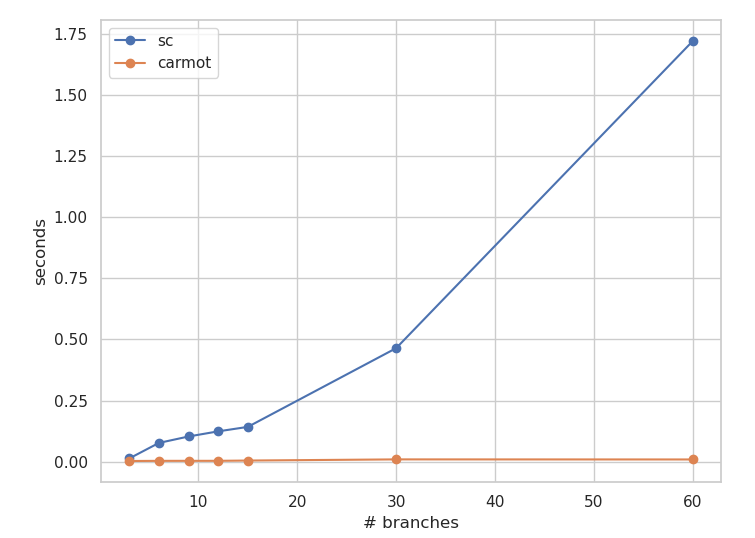
\includegraphics[scale=0.3]{Figures/latency}
\caption{Latency of collaborative editing operations under \quark vs
  executing them with strong consistency (SC). }
\label{fig:latency}
\end{figure}

To measure the impact of \quark runtime on user writes, we measure the
latency of the \C{write} operation, which includes for the time spent
merging the user version with the current version, and persisting the
resultant version to the store. We conduct the experiments on a
three-node cluster of \C{i3.large} machines in Amazon \C{us-west2}
data center. Each user connects to one of the machines and performs
1000 edits in succession, saving the document after each edit. We
progressively increase the number of concurrent users editing the
document from 3 to 60 and measure the impact of the increased
concurrency on write latency. Fig.~\ref{fig:latency} shows the median
latency values. As evident from the figure, latency of \quark writes
remain more-or-less constant with the median latency around 0.008s.
The maximum latency ever measured for a \quark writes is 0.016s.
Notably, latency remains an order of magnitude less than the time
between consecutive edits (0.25s), making it hard to perceive.
Fig.~\ref{fig:latency} also plots the latency values for the baseline
``SC'' approach which achieves convergence by synchronizing each
operation, i.e., executing under strong consistency (SC). The SC write
latency increases super-linearly with the median value of 1.76s for 60
concurrent editors. The maximum latency measured for an SC write is
9.02s, which is considerably more than the inter-edit latency of
0.25s. The experiment confirms the theory that convergence does not
come at the cost of latency in
\quark.

\begin{figure}[ht]
  \centering
    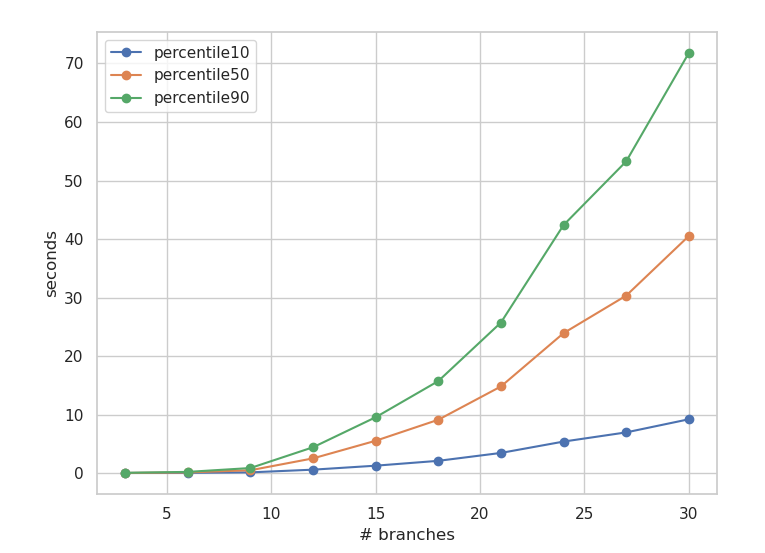
\includegraphics[scale=0.3]{Figures/staleness}
\caption{Staleness increases as the number of concurrent editors
  increase.}
\label{fig:staleness}
  \vspace*{-0.2in}
\end{figure}

\quark system replicates the contents of each branch across all the
replicas as fast as the network allows. However, for a user $A$ to
see the changes made by the other user $B$, the changes have to be
reflected in $A$'s local version, which can only happen through a
merge operation. Since \quark synchronizes merge operations globally,
it induces additional delay before $A$ can see $B$'s changes. We call
this additional delay \emph{staleness} as with the progression of
time, $B$'s version known to $A$ becomes increasingly stale. At the
system-level, an increase in staleness effectively delays the
convergence (but doesn't preempt it, as proved by
Theorem~\ref{thm:progress}). To understand the staleness behavior in
\quark, we repeat the collaborative editing experiment, this time
measuring the staleness value at every merge. We do this by annotating
every version $v$ with the timestamp $t$ of its creation time. When
$v$ is is merged into a remote branch $b$ at a later time $t'$, the
difference $t' - t$ denotes the staleness of $v$ w.r.t the new version
on $b$. Multiple such staleness measurements are recorded for each
experiment to compute the 10th, 50th, and 90th percentile
values. Fig.~\ref{fig:staleness} shows the results. While
staleness remains in the order of milliseconds with fewer ($\leq 9$)
concurrent users, it increases super-linearly as we increase the
number of collaborators in the multiples of 3 until 30. While
increased staleness is inevitable in our approach due to synchronized
merges, we believe the increase can be contained by choosing the order
of merges to avoid the ``starvation'' of some branches. Note that
relaxing the linearizability constraint on merges would completely
eliminate the staleness overhead, but the resultant Git-like system
fails to converge due to anomalous executions described in
Sec.~\ref{sec:motivation}\footnote{
  Git admits anamolous version history graphs where two branches can
  have the same set of commits and yet differ in their final version.
  Supplementary material describes two such cases we observed on
  Github.}. 

Our experiments bring to the fore an inherent tradeoff among the
competing concerns of RDTs, namely (\rom{1}). The ease of programming
convergence, (\rom{2}) Latency, and (\rom{3}).  Staleness. While CRDTs
try to optimize for latency and staleness, they require a significant
amount of development and verification effort to be expended to ensure
convergence~\cite{kleppmann2017}. In contrast, \quark lets developers
derive convergent-by-construction RDTs from ordinary data data types
that are optimized for latency, but incur a staleness overhead that
delays the time to convergence. 


